


In this part of the homework we use the QR-factorization to solve a square ill-conditioned system. We use the given function \texttt{illposed.m} to generate an ill-conditioned system of size 8. 

\paragraph*{a) Estimate condition number of a linear system}

Given the matrix $A$, we can introduce a perturbation $b+\Delta b$ to estimate the condition number of $A$ with 
$$\dfrac{\parallel \Delta x \parallel_2}{\parallel x \parallel_2}\leq\kappa (A)\dfrac{\parallel \Delta b \parallel_2}{\parallel b \parallel_2}.$$

We took a large number of random perturbations and kept the one that gave the worst estimation of the condition number. The estimation of the condition number for the matrix $A$ 

\begin{table}[hb]
\centering
\begin{tabu}{|c|c|}
\hline 
\texttt{cond(A)} & \texttt{estimateCond(A)} \\ 
\hline 
1.5137e+12 & 2.7591e+11 \\ 
\hline 
\end{tabu}
\caption{Estimated condition number of A compared with Matlab}
\end{table} 
It is clear that we find a lower bound of the exact condition number since we can only try a finite number of perturbations.


\paragraph*{b) Approximate solution of ill-posed system}

\begin{center}
\begin{tabular}{|c|c|c|c|c|c|}
\hline 
rank & $\parallel E \parallel$  & $\parallel res \parallel$ &  cond(R11) & estimationCond(R11) & $\parallel \hat{x} \parallel$ \\ 
\hline 
8 & /                  & $10^{-15}$     & $1.68*10^{12}$ & $0.79*10^{12}$      &  1.377 \\ 
\hline 
7 & 5                  & $3.5*10^{-12}$ & $0.0026*10^{12}$ & $0.0013*10^{12}$ &  1.418 \\ 
\hline 
6 & $2.2*10^{3}$         & $2158*10^{-12}$ & $10.025$        & 4.156 &  1.539 \\ 
\hline 
5 & $0.4305*10^{12}$     & 0.2912       & 5.976  & 4.167 &  1.772 \\ 
\hline 
\end{tabular} 
\end{center} 





\begin{figure}
\begin{center}
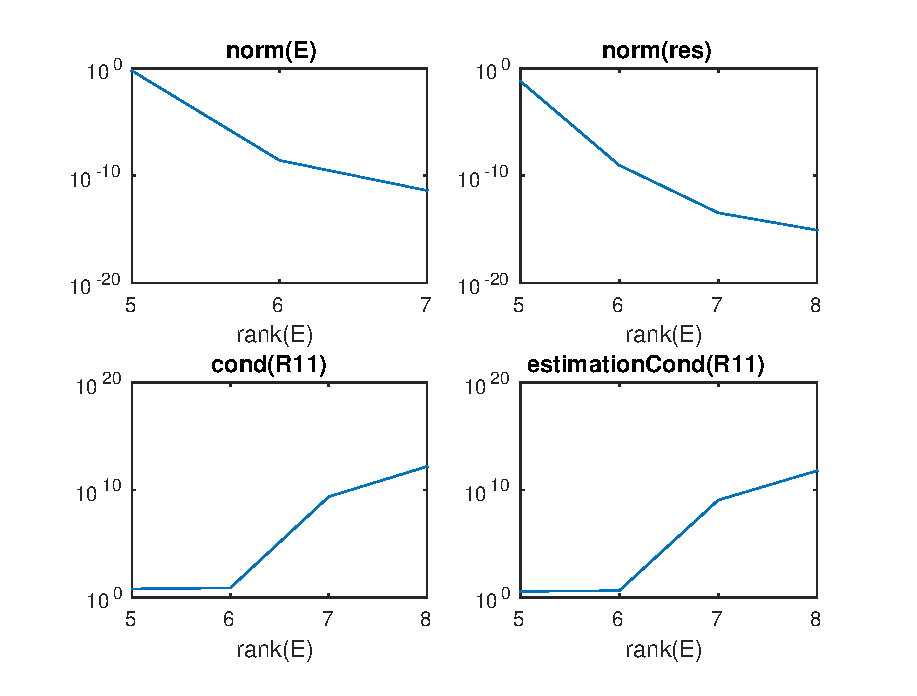
\includegraphics[scale=0.7]{qrPlot.eps}
\caption{Numerical relations as a function of the rank $r$}
\label{lsp}
\end{center}
\end{figure}

\FloatBarrier







